%%=============================================================================
%% Analyse
%%=============================================================================

\chapter{\IfLanguageName{dutch}{Analyse}{Analysis}}%
\label{ch:analyse}
\section{\IfLanguageName{dutch}{Casusbedrijf}{Casusbedrijf}}%
\label{sec:casusbedrijf}
Het casusbedrijf Liantis is een middelgrote onderneming met meer dan 2000 medewerkers. Het vindt historische zijn roots in 1942 als ADMB Sociaal Bureau, waar het werd opgericht om ondernemers te ondersteunen in kader van sociale zaken en personeelsbeleid als sociaal secretariaat. Een latere fusie in 2018 met Zenito, een vzw die diensten aanbood aan beginnende zelfstandigen en Previkmo, een externe dienst voor preventie en bescherming op het werk, creëerde de huidige dienstengroep Liantis.\newline

Deze fusie ging uiteraard gepaard met een grote oefening rond procesbeheer en IT. De drie afzonderlijke IT-departementen werden, samen met hun portfolio aan applicaties, gefuseerd tot een IT-bedrijf specifiek gericht op ontwikkeling, implementatie en onderhoud van het IT-landschap van de volledige dienstengroep. Dit verklaart dan ook de hoge hoeveelheid aan in-house ontwikkeling. Elk afzonderlijk bedrijf had immers voor zijn eigen werking software ontwikkeld en ze waren allen te kleinschalig om grotere out-of-the-box systemen te implementeren. Dit versprokkeld IT- en proceslandschap blijft voor dit bedrijf tot op de dag van vandaag wegen op zijn groei en bemoeilijkt het moderniseren van zijn werking.
\section{\IfLanguageName{dutch}{Functionele Vereisten}{Functionele Vereisten}}%
\label{sec:functionele vereisten}
\subsection{\IfLanguageName{dutch}{Opzet}{Opzet}}%
\label{subsec:opzet func}
Om te ontdekken welke mogelijke toepassingen dit systeem kan hebben, werden workshops georganiseerd om een aantal stakeholders langs business kant te bevragen. De workshops werden als volgt georganiseerd:
\begin{itemize}
  \item De stakeholders kregen een brede uitleg met wat proces monitoring en orkestratie is met voorbeelden vanuit het werkveld. Gelet op hun ervaringen met andere soorten automatisatie pakketten konden ze snel begrijpen hoe dergelijk systeem in theorie werkt.
  \item De stakeholders werden gevraagd om in groep te brainstormen rond mogelijk praktische applicaties van dergelijke systemen binnen het bedrijf. Ze kennen immers de huidige producten het beste als domeinexperten.
  \item De stakeholders moesten post-its met hun theoretische use-cases voor zowel monitoring als orkestratie op het bord zetten met eveneens hoe zij dit in praktische implementaties zouden gerealiseerd willen zien binnen de bestaande producten.
\end{itemize}
De bedoeling van deze workshop was enerzijds om te polsen welke noden dit systeem zou kunnen vervullen, maar ook om te kijken waar het zou kunnen inhaken op de al bestaande systemen. Als bepaalde systemen een duidelijke nood hebben, dan zou het proces die deze systemen hanteert een sterk kandidaat-proces zijn voor de proof-of-concept. Als stakeholders werd gekozen om een business architect, een business owner, een productmanager en een aantal product owners te betrekken bij deze workshops. Hierdoor was er een goede mix van management, architectuur en domeinkennis beschikbaar, maar is er ook een praktische link naar het IT-landschap aanwezig voor input.


\subsection{\IfLanguageName{dutch}{Workshop Proces Monitoring}{Workshop Proces Monitoring}}%
\label{subsec:workshop proces monitoring}
\begin{center}
  \captionsetup{type=figure}
  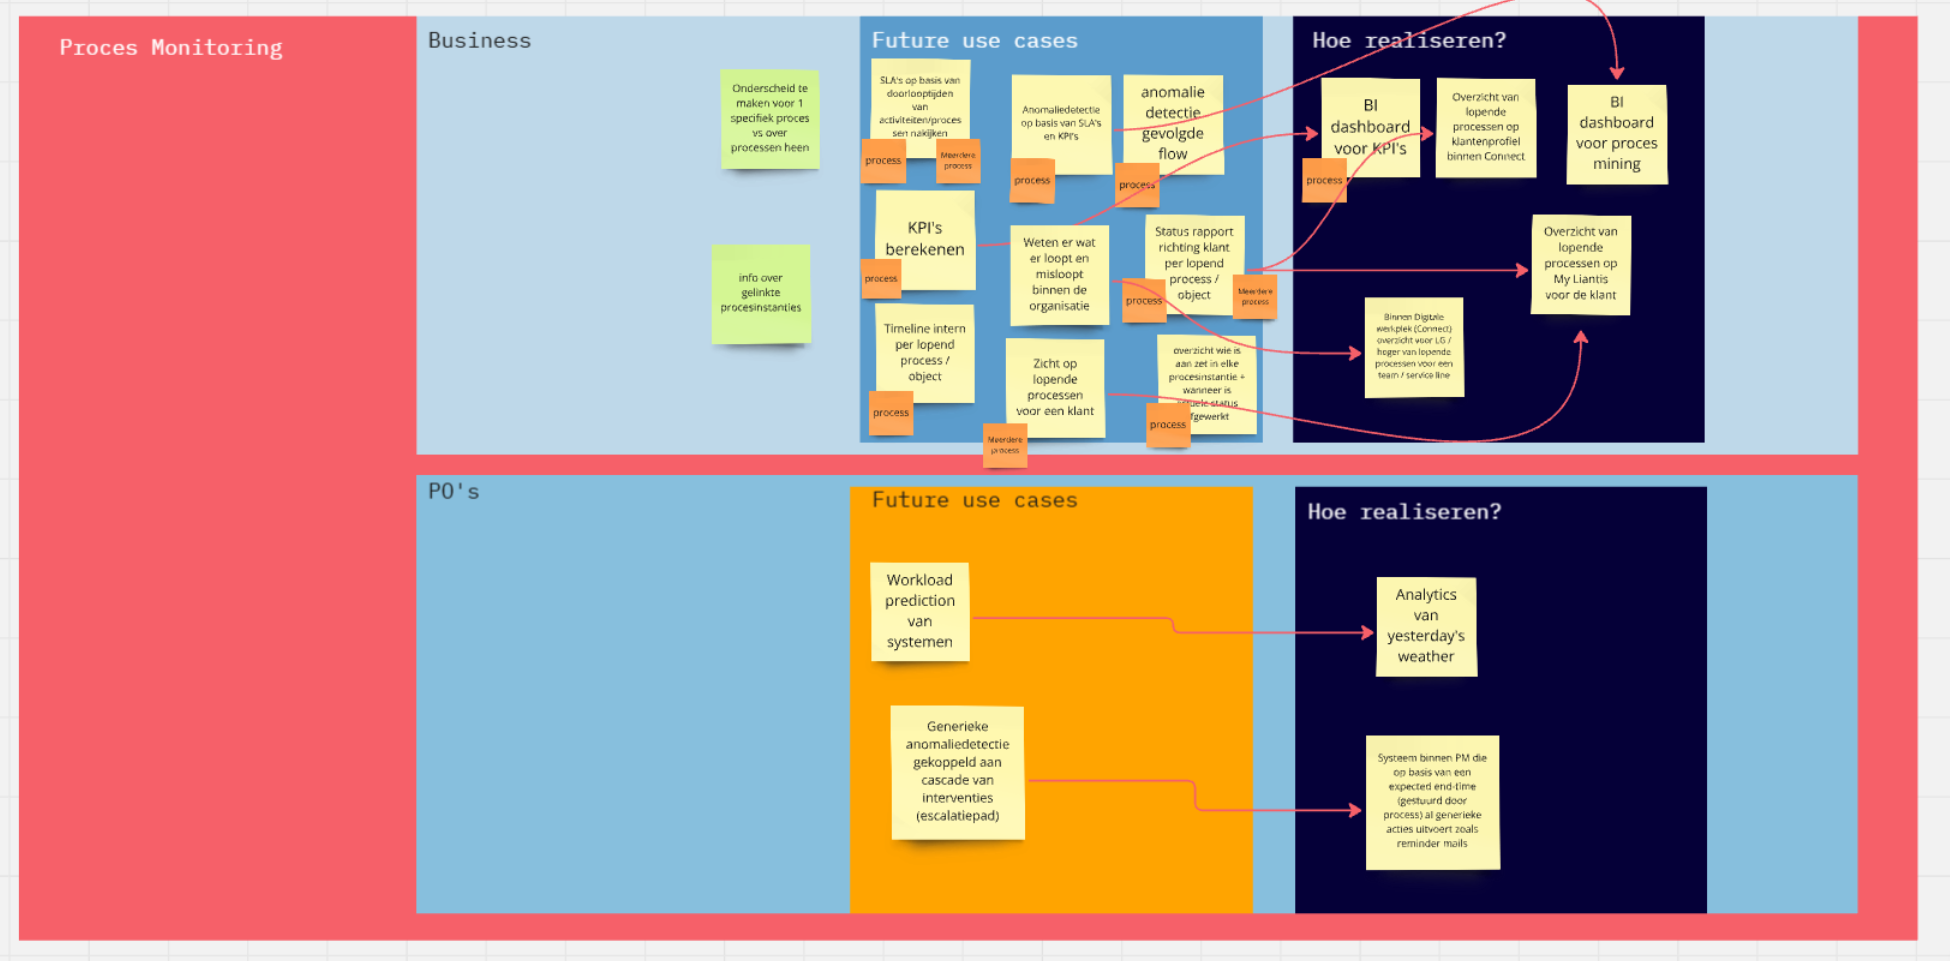
\includegraphics[width=1.0\linewidth]{PM.png}
  \captionof{figure}[Whiteboard voor de proces monitoring workhop]{Whiteboard voor de proces monitoring workhop}
\end{center}
De workshop proces monitoring onthulde een aantal mogelijke use-cases met bijhorende realisaties binnen het IT-landschap.\newline

De eerste grote use-case is de vraag om op basis van de monitoring zowel de klant als bevoegde manager op de hoogte te houden van het lopend proces. Business zou hierbij willen dat er een timeline is van elk lopend proces, dat het duidelijk is wie momenteel bezig is aan welke stap binnen elk instantie van het proces en of bepaalde mijlstenen van het proces bereikt zijn. Een subset van deze informatie zou nuttig zijn om de klant in real-time te informeren over het lopend proces. Dit zou enerzijds gerealiseerd kunnen worden met een statuspagina binnen het klantenportaal MyLiantis per klant en anderzijds een diepere leidinggevende view binnen de Digitale Cockpit waar de manager een helikopterzicht zou krijgen van de werkzaamheden van het team. \newline

Een tweede grote use-case is de vraag naar betere rapportage en complexe business intelligence. Business zou graag een dashboard willen waar statistische data rond processen beschikbaar is zoals doorlooptijden, maar ook waar key performance indicatoren gemeten worden. Op basis van deze data zou ook de werklast van elke medewerker kunnen gevolgd worden om ervoor te zorgen dat die efficiënt benut wordt, maar ook om overwerk te vermijden. Op basis van de groeiende historische data zou men ook aan forecasting willen doen en zelfs de verwachte aflooptijd willen kunnen berekenen van een lopend proces. Tot op heden is dergelijk dashboard niet voorhanden. \newline

Een derde grote use-case is anomaliedetectie. Op basis van vooraf bepaalde servicelevel overeenkomsten per activiteit moet het mogelijk zijn om bij een potentiële breuk op deze overeenkomsten automatisch de juiste mensen te contacteren en via escalatiepaden remediërende acties in gang te steken zoals reminder-e-mails of herprioretisering van taken.\newline

Het is duidelijk dat er veel mogelijke toepassingen zijn voor de data die proces monitoring zou capteren mits deze op een correcte manier beschikbaar gesteld kan worden via nuttige API’s. Enerzijds zou dit real-time status info voor business en klanten kunnen faciliteren en anderzijds zou dit verregaande rapportage op basis van business intelligence toelaten met eventuele anomaliedetectie. Opvallend is dat het klantenportaal MyLiantis vaak terugkeert in de antwoorden. Dit portaal heeft als centraal proces de onboarding van nieuwe medewerkers bij klanten. Dit doet vermoeden dat het onboarding proces voor nieuwe medewerkers van klanten een interessant kandidaat proces kan zijn voor de proof-of-concept.

\subsection{\IfLanguageName{dutch}{Workshop Proces Orkestratie}{Workshop Proces Orkestratie}}%
\label{subsec:workshop proces orkestratie}
\begin{center}
  \captionsetup{type=figure}
  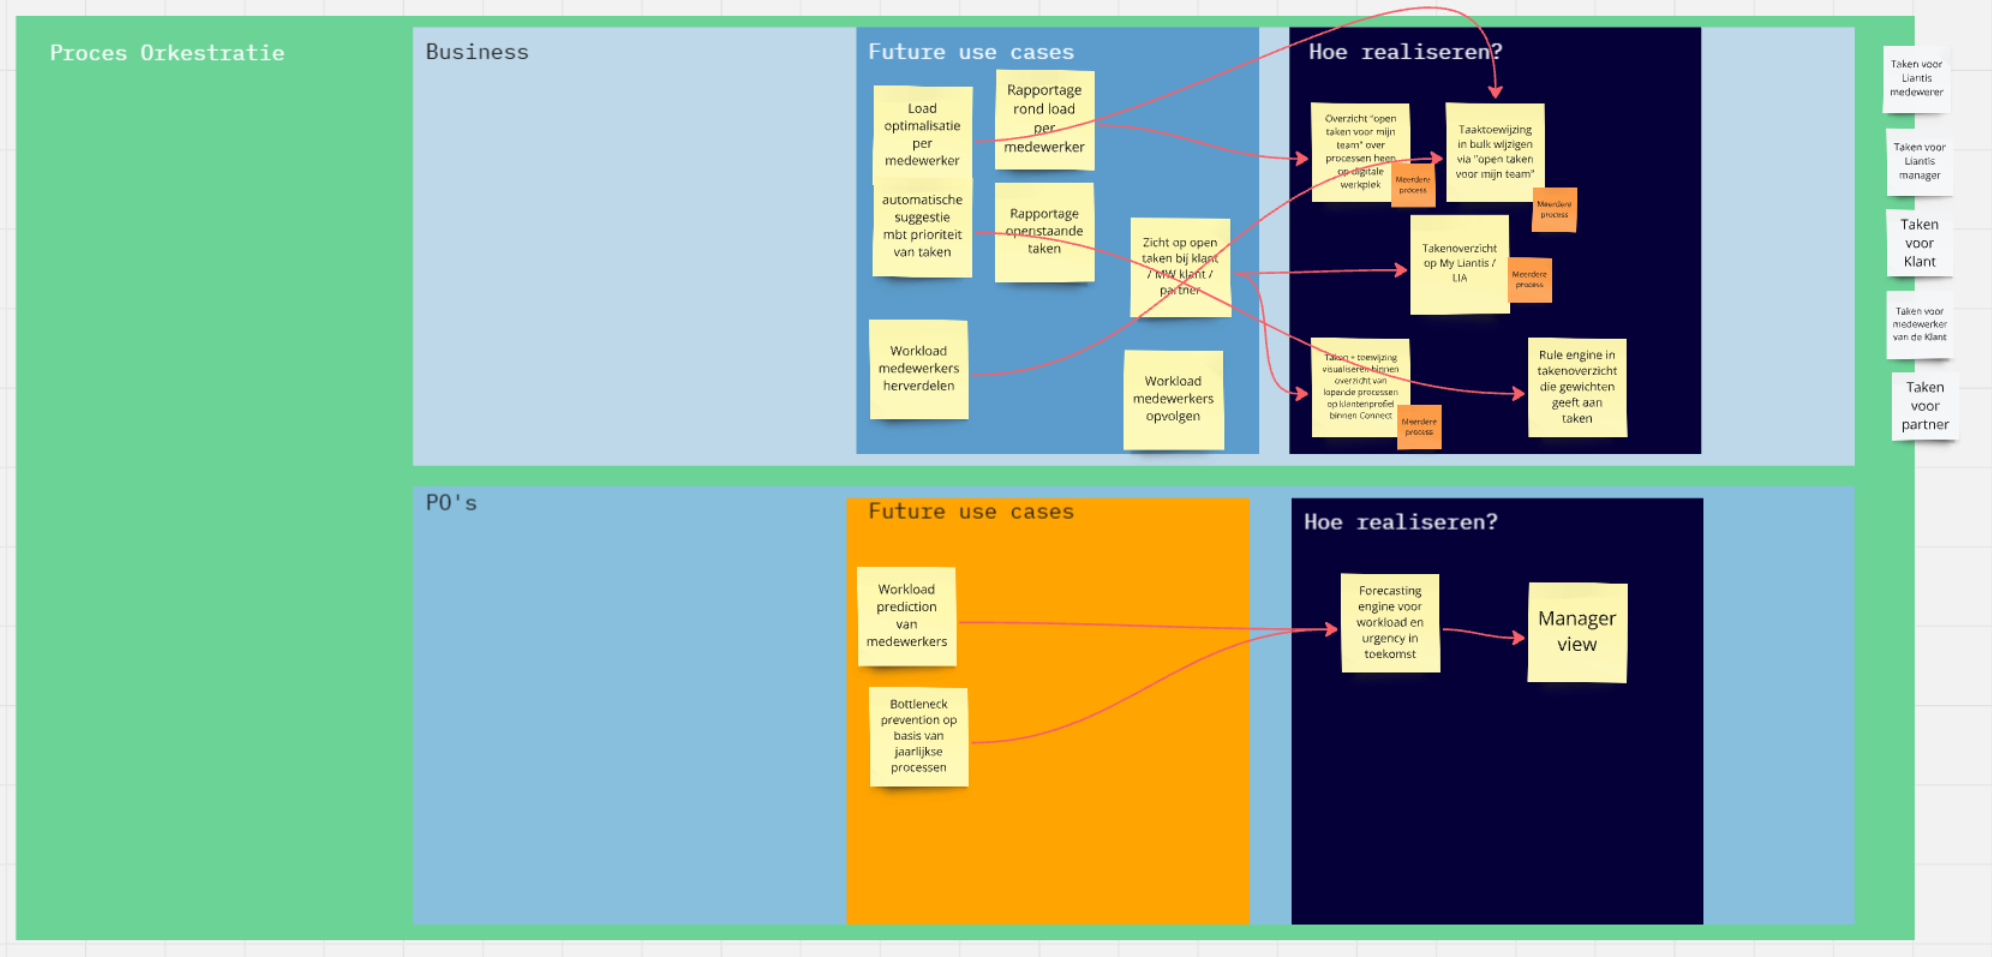
\includegraphics[width=1.0\linewidth]{PO.png}
  \captionof{figure}[Whiteboard voor de proces orkestratie workhop]{Whiteboard voor de proces orkestratie workhop}
\end{center}

De workshop proces orkestratie onthulde een aantal mogelijke use-cases met bijhorende realisaties binnen het IT-landschap. \newline

De eerste grote use-case is de vraag naar een manier om een slimme en data-gestuurde volgorde in de uitvoering van taken door medewerkers te implementeren met oog op werklast optimalisatie. Het systeem zou op het juiste moment de juiste taak moeten suggereren voor elke medewerker op basis van het aantal openstaande dossiers, de relevante servicelevel overeenkomsten en hun huidige werklast. Een mogelijke realisatie hiervoor zou dan een takenoverzicht per dossier zijn in het klantenportaal MyLiantis en een persoonlijke takenlijst in de Digitale Cockpit van elke medewerker. \newline

Een tweede use-case zou een manier moeten zijn om in bulk te kunnen ingrijpen op dit systeem als manager indien er speciale situaties zich voordien waar het systeem geen rekening mee kan houden op basis van de info vanuit het proces en de monitoring. Een voorbeeld hiervan zijn VIP-klanten of taken die omwille van speciale uitzonderingsevents zoals wettelijke veranderingen opeens een harde deadline krijgen. Dit heeft twee mogelijke implementaties. Enerzijds zou de manager dit imperatief willen kunnen doen door naar een specifiek dossier te gaan en daar de volgende openstaande taak binnen het proces toe te wijzen aan een medewerker. Anderzijds zou een manager specifieke dossiers of zelfs klanten willen kunnen prioriteren zodat hun taken of dossiers voorrang krijgen op die van anderen. Een mogelijke realisatie hiervoor zou een uitbreiding zijn op de voorgenoemde manager-view in de Digitale Cockpit waarbij de manager naast de rapportage vanuit de proces monitoring ook deze aanpassingen zou kunnen doen voor dossiers die binnen zijn portfolio passen. \newline

De nood aan een taakoverzicht voor medewerkers is een heel bekende bij bedrijven en is een van de features waar de systemen van IBM en Bizagi mee uitpakken. Dit zou dan ook een heel basic vereiste moeten zijn. De nood om taken imperatief te kunnen toewijzen aan medewerkers is ook zeker te verantwoorden. Een actieve manager zal de prioriteiten altijd beter kunnen inschatten dan een automatisch systeem. Prioriteiten voor dossiers en klanten aanpassen is echter een veel complexere eis omdat dit rechtstreeks het algoritme van de executie engine zou affecteren. Dit zou alvast iets zijn voor een verdere iteratieve cyclus en niet voor een proof-of-concept of MVP. \newline

Bij deze workshop kwam het klantenportaal MyLiantis nogmaals een aantal keer aan bod. Dit bevestigt dat het onboarding proces een interessant kandidaat proces kan zijn voor ons.

\section{\IfLanguageName{dutch}{Technische Vereisten}{Technische Vereisten}}%
\label{sec:technische vereisten}
\subsection{\IfLanguageName{dutch}{Opzet}{Opzet}}%
\label{subsec:opzet tech}
Nu de functionele vereisten veel duidelijker zijn, komen de technische vereisten en niet-functionele vereisten aan bod. Om deze te capteren werd een brainstormingsessie georganiseerd met een van de systeem architecten van het casusbedrijf die de materie rond proces monitoring en orkestratie goed kent. De eerder gevonden vereisten werden besproken en op basis hiervan werd nagegaan aan welke vereisten het systeem minimaal zou moeten voldoen om te passen binnen het IT-landschap van het bedrijf.
\subsection{\IfLanguageName{dutch}{Brainstorming Sessie met Systeem Architect}{Brainstorming Sessie met Systeem Architect}}%
\label{subsec:brainstorming sessie met systeem architect}
Het casusbedrijf gebruikt in al zijn softwareapplicaties een combinatie van Spring Boot voor de back-end en Angular voor de front-end. Qua programmeertalen zijn de standaardtalen enerzijds Java en anderzijds Type-Script. Op vlak van databasissen is de standaard vooral traditionele SQL, hoewel er geen probleem is om No-SQL opties te gebruiken zoals de documentstore Cosmos DB. Andere No-SQL opties zoals een graaf databasis zijn eerder een uitzondering, maar worden wel ondersteund. \newline

Architecturaal gebruikt het bedrijf vooral een microservices architectuur waarbij een applicatie traditioneel bestaat uit een of meerdere back-ends met bijhorende databasis, een gateway die de toegang tussen back-ends onderling en front-ends medieert en een front-end waar de eindgebruikers in werken. De microservices communiceren met elkaar op basis van REST API-calls indien ze deel uitmaken van dezelfde applicatie of via berichten en eventing als ze dat niet doen. Afnemers van data mogen ook rechtstreeks API-calls uitvoeren via de gateway. De berichten worden geregeld via RabbitMQ, een message broker die het AMQP-standaard ondersteund, terwijl events geregeld worden via Azure Event Hubs.\newline

Infrastructureel zit het casusbedrijf nog volop in zijn transitie naar de cloud. Een deel van de software draait on-premise op een datacenter met Apache Tomcat servers terwijl merendeel van de software draait op Microsoft Azure Cloud in Docker containers. Voor de on-premise software wordt de versionering gedaan via Bitbucket met Jenkins als ci/cd pipeline terwijl de toepassingen in de cloud op Github staan met Github actions als ci/cd pipeline. Voor een zeer klein deel legacy applicaties wordt de versionering en configuratie nog gedaan via Subversion, hoewel deze volop uitgefaseerd worden. \newline

Dit overzicht geeft ons al een duidelijk beeld van waar de software aan gaat moeten voldoen. Als databasis is vrije keuze tussen SQL of een documentstore per back-end. De back-end moet in Java gecodeerd zijn met Spring Boot als framework. Indien er een front-end of meerdere back-ends aanwezig zijn, is er nood aan een gateway om de connectie de mediëren. Indien er een front-end is, dan moeten deze in Type-Script geschreven worden met Angular als framework. Inkomende communicatie vanuit andere systemen gaat via berichten. Afnemers hebben een duidelijke REST-API nodig. \newline

Gelet op de vereisten van business is voor de proof-of-concept een front-end niet aan de orde. Het is immers een vereiste dat de informatie uit beide systemen ingebouwd wordt in al bestaande front-ends. Rapportage gebeurt ook via business intelligence dashboards. Het is dus vooral belangrijk dat de back-end systemen duidelijk API’s hebben voor afnemende systemen en business intelligence. Dit betekent ook dat een gateway niet aan de orde zal zijn. Hoewel er argumenten zijn om te werken met een documentstore, primeert de nood aan consistente en juiste data boven alles. SQL is ook de regel binnen het landschap waardoor No-SQL een nutteloze complexiteit lijkt.  De technische scope is nu dus veel duidelijker.
\section{\IfLanguageName{dutch}{Niet-functionele Vereisten}{Niet-functionele Vereisten}}%
\label{sec:niet-functionele vereisten}
\subsection{\IfLanguageName{dutch}{Overlopen NFR-checklist met Systeem Architect}{Overlopen NFR-checklist met Systeem Architect}}%
\label{subsec:overlopen nfr-checklist met systeem architect}
Het casusbedrijf meet elke potentiële applicatie aan een aantal niet-functionele vereisten. Hierbij moet er altijd het minimum bereikt worden van ISO-norm 25010 als standaard voordat deze toegelaten kan worden als applicatie binnen het IT-landschap. Afhankelijk van de aard van het product zullen de vereisten strenger zijn. Standaard moet de trekker van een project een NFR-checklist invullen voor om het even welk softwareproject mag opgestart worden. Dit moet dan door de architecten gevalideerd worden zodat er minstens aan de minimale vereisten wordt voldaan. Deze checklist werd tijdens de brainstorming sessie ook ingevuld. Voor een proof-of-concept zijn de eisen veel lager gezien het de bedoeling is dat dit tijdens het eigenlijk project wordt behaald. Het theoretisch eindproduct zou echter moeten voldoen aan de volgende niet-functionele vereisten. \newline

Availability is als vereiste verbonden aan hoe kritisch het business proces is dat de software ondersteunt en wat de schade voor het bedrijf is indien de werking van de software verstoord wordt. Uit voorgaande workshops zag business de software enerzijds als informatief voor klant en de manager, anderzijds als sturend voor de medewerkers. Het neergaan van de software zou ertoe leiden dat een aantal processen zwaar vertraagd tot onuitvoerbaar zouden zijn. Hierdoor zou de software bestempeld worden als bedrijf kritisch. Qua availability moet deze software dus tijdens de kantooruren zo goed als 99,999\% van de tijd beschikbaar zijn. Het bedrijf volgt hier het “Five Nines”-principe. He is even streng qua foutbestendigheid. De software moet zichzelf kunnen remediëren op basis van zijn interne logica en data op basis van back-ups. \newline

Performantie is ook belangrijk gezien vertragingen rechtstreeks geld kosten. De algemene verwachting binnen het bedrijf voor synchrone processen is een responsetijd van 100 milliseconden en voor asynchrone processen is dit 30 seconden. Op vlak van presentatie is mag de laadtijd van een scherm niet boven 1 seconde zijn en voor acties binnen een scherm is de verwachting een responstijd van maximaal 500 milliseconden. Dit is algemeen zo voor alle applicaties binnen het bedrijf.\newline

In kader van configureerbaarheid en beheerbaarheid moet het product een externe configuratie kunnen aanvaarden. Een gebruiker hoort de data voor proces monitoring niet van buitenaf te kunnen beheren gezien het systeem zelf zijn data genereert. Ingrijpen op taken binnen de orkestratie zou dan weer wel moeten via een duidelijke UI of API die mogelijke acties van eindgebruikers limiteert tot het essentiële. De data zelf moet voor een gewone lezer niet zomaar uit te lezen zijn en moet, waar mogelijk, werken met generische referenties zodat enkel een ander systeem dit correct kan interpreteren en tonen aan de gebruiker. Dit houdt ook in dat het systeem input moet verwerken van om het welk proces of systeem binnen het bedrijf zonder te weten wat de data zelf representeert. De uiteindelijk vertaling is de verantwoordelijkheid van de afnemer. \newline

Op vlak van observability is er minimaal een technische monitor rond de infrastructuur waar de software op draait voor status, CPU-gebruik, geheugen-gebruik, disk I/O, disk ruimte en netwerk I/O aanwezig. Dit zit al ingebouwd op de cloud containers en moet dus in meeste gevallen niet actief gebouwd worden. Er moet ook duidelijke interne logging zijn die extern aggregeerbaar is via tooling zoals Dynatrace of Grafana. \newline

Security is een belangrijk onderwerp. Het casusbedrijf heeft daarom een intern authenticatie module voor elke login en endpoint. Er moet ook gelaagde autorisatie met rollen ingevoerd zijn in de software. Als de mogelijkheid bestaat om via menselijke interactie de data aan te passen, dan moet er een historische audit log bijgehouden worden waarin staat wie welke data wanneer aanpaste met de oude en nieuwe waarde in de log. 